%\documentclass[aps,prb,superscriptaddress,showpacs,reprint]{revtex4-1}
\documentclass[aps,prb,showpacs,reprint]{revtex4-1}
\usepackage{fullpage}
\usepackage{amsfonts}
\usepackage{amssymb}
\usepackage{amsmath}
\usepackage{hyperref}
\usepackage{graphicx}% Include figure files
\usepackage{epstopdf}
\usepackage{subfig}
\usepackage[normalem]{ulem}
\begin{document}
%\usepackage{setspace}\doublespace
\title{Competition between BCS-pairing and moth eaten effect in BEC-BCS crossover}
\author{Guojun Zhu}
\affiliation{Department of Physics, University of Illinois at Urbana-Champaign, 1110 W Green St, Urbana, IL, 61801}
\author{Monique Combescot}
\affiliation{Institut des NanoSciences de Paris, Universite Pierre et Marie Curie, CNRS, Tour 22, 4 place Jussieu, 75005 Paris }
\affiliation{Department of Physics, University of Illinois at Urbana-Champaign, 1110 W Green St, Urbana, IL, 61801}

\newcommand{\vk}{\ensuremath{\mathbf{k}}}
\newcommand{\vK}{\ensuremath{\mathbf{K}}}
\providecommand{\vr}{\ensuremath{\mathbf{r}}}
%\newcommand{\vec}[1]{\ensuremath{\mathbf{#1}}}

\newcommand{\gk}{\ensuremath{{g}(\mathbf{k})}}

\newcommand{\vp}{\ensuremath{\mathbf{p}}}
\newcommand{\gp}{\ensuremath{{g}(\mathbf{p})}}

\newcommand{\vq}{\ensuremath{\mathbf{q}}}

\newcommand{\Fo}{\ensuremath{\mathbf{F_0}}}


\newcommand{\E}{\ensuremath{\mathbf{E}}}
\newcommand{\A}{\ensuremath{\mathbf{A}}}
\newcommand{\J}{\ensuremath{\mathcal{J}}}

\newcommand{\ket}[1]{\ensuremath{\left|#1\right>}}
\newcommand{\bra}[1]{\ensuremath{\left<#1\right|}}

\newcommand{\twoe}{\ensuremath{2\epsilon_\vk-\E_1}}

\newcommand{\nth}[1]{\ensuremath{\frac{1}{#1}}}

\newcommand{\br}[1]{\ensuremath{\left(#1\right)}}
\newcommand{\mbr}[1]{\ensuremath{\left[#1\right]}}
\newcommand{\bbr}[1]{\ensuremath{\left\{#1\right\}}}


\newcommand{\tk}{\ensuremath{\tilde{k}}}

\newcommand{\kp}{\ensuremath{\ket{\Psi}}}

\newcommand{\av}[1]{\ensuremath{\bigl<{#1}\bigr>}}
\newcommand{\avs}[3] {\av{#1{\lvert{#2}\rvert}#3}}
\newcommand{\avv}[2][\nu] {\avs{#1}{#2}{#1}}
\newcommand{\avt}[2]{\av{{#1}|{#2}}}
\newcommand{\avtu}[1]{\av{T_\tau#1}}

\newcommand{\Bop}{\ensuremath{\mathbf{B_0^+}}}
\newcommand{\Bmp}{\ensuremath{\mathbf{B_m^+}}}
\newcommand{\Bnp}{\ensuremath{\mathbf{B_n^+}}}
\newcommand{\Bo}{\ensuremath{\mathbf{B_0}}}
\newcommand{\Bopn}{\ensuremath{\mathbf{{B_0^+}^n}}}
\newcommand{\Bon}{\ensuremath{\mathbf{{B_0}^n}}}


\newcommand{\zmatrix}{\ensuremath{\br{\begin{smallmatrix}0&0\\0&0\end{smallmatrix}}}}
\newcommand{\fmtrx}[4]{\ensuremath{\br{\begin{smallmatrix}#1&#2\\#3&#4\end{smallmatrix}}}}
\newcommand{\smtrx}[6]{\ensuremath{\br{\begin{smallmatrix}#1&#2\\#3&#4\\#5&#6\end{smallmatrix}}}}

\newcommand{\vz}{\ensuremath{v^{\beta\alpha}_{\vk,\vk}}}


\providecommand{\abs}[1]{\ensuremath{\lvert{#1}\rvert}}

\newcommand{\sg}[1][1]{\ensuremath{\sigma_\frac{#1}{2}}}

\newcommand{\rhof}{\ensuremath{\rho(\ef)}}
\newcommand{\omt}{\ensuremath{\tilde{\Omega}}}
\newcommand{\cht}{\ensuremath{\tilde{\chi_0}}}
\newcommand{\Atl}{\ensuremath{\abs{A}^{2l}}}
\newcommand{\ef}{\ensuremath{\epsilon_F}}

\newcommand{\lca}{\ensuremath{\ln\br{1+\frac{\cht}{\alpha}}}}

\newcommand{\com}[2]{\ensuremath{\mbr{#1,#2}}}
\newcommand{\D}{\ensuremath{\mathit{D}}}
\newcommand{\dg}{\ensuremath{\dagger}}
\newcommand{\nG}{\ensuremath{\hat{\mathcal{G}}^{-1}}}

\providecommand{\lvk}{\ensuremath{1/\vk_F}}
\providecommand{\hm}{\ensuremath{\frac{\hbar^2}}{2m}}
\providecommand{\pdiff}[2]{\ensuremath{\frac{\partial{#1}}{\partial{#2}}}}
\providecommand{\dpdiff}[2]{\ensuremath{\frac{\partial^2{#1}}{\partial{{#2}^2}}}}

\providecommand{\H}{\ensuremath{\mathcal{H}}}
\providecommand{\wt}[1]{\widetilde{#1}}

\providecommand{\eef}[1]{Eq. (\ref{#1})}

\providecommand{\sch}{{Schr\"{o}dinger }}

\providecommand{\sgn}{\ensuremath{\text{sgn}}}
\newcommand{\Arctg}{\ensuremath{\text{Arctg}}}

\providecommand{\comm}[1]{\textit{\scriptsize \uwave{(#1)}}}
\newcommand{\td}{{\ensuremath{{\text{(2D)}}}}}
\newcommand{\sd}{{\ensuremath{{\text{(3D)}}}}}
\newcommand{\Arctg}{\ensuremath{\text{Arctg}}}



\numberwithin{equation}{section}
\begin{abstract}
We study the evolution of solution to reduced BCS hamiltonian from single pair to infinite amount of pairs in thermodynamic limit.  We observe that absolutely amount of energy-saving due to pairing decreases while pair number increases because the phase space for each additional pair gets smaller (moth-eaten effect).  However, comparing to the increase of kinetic energy as free Fermi gas, this decrease is smaller at first and only dominates  when total number of particles is close to the total available states.  
\end{abstract}
\maketitle
\section{Introduction}
It was known for a long time that a 3D system having a weak attractive potential cannot sustain a bound-state.  In 1956, Cooper showed that in the presence of a frozen Fermi sea, a pair of electrons with opposite spin can form a bound-state of zero total momentum  no matter how weak the attraction is\cite{Cooper}.  This state actually is indeed a many-body state because the  Fermi sea, even if it does not interact through the reduced BCS potential,  is essential for the formation of ``two-body'' bound state.   The next year, Bardeen, Cooper and Schrieffer introduced a many-body ansatz which is an extension of this single pair ``bound state'' and showed that this ansatz gives an intricate many-body state with lower energy than free Fermi gas with arbitrarily weak attraction\cite{BCS} for the same reduced BCS hamiltonian.  They used a particle-number non-conserved ansatz in a grand-canonical ensemble.  Nevertheless, the reduced BCS model also has a frozen Fermi sea in the core. Later,   Gor'kov and Melik-Barkhudarov showed that the frozen Fermi sea is not necessary and the same idea works with a renomalized attraction measured by low energy scattering amplitude\cite{Gorkov}.   Furthermore, Eagles\cite{Eagle}, Leggett\cite{LeggettCrossover}, Nozi\`{e}res and Schmitt-Rink\cite{Nozieres} extended the BCS pairing idea and bridged Cooper pairing and molecular BEC. There they used the model without a frozen Fermi sea as core and employed the full k-space.  All these lead to an interesting question that how the solution for the same hamiltonian evolves from one-pair, where there might be no bound state, to infinite number of pairs, where a many-body bound solution always exists.  Nevertheless, the particle non-conserved nature of the BCS ansatz makes it inherently many-body, which is quite difficult to connect to one-pair solution.  

Five years after BCS, Richardson showed that a number-conserved eigenstate exists for the reduced BCS Hamiltonian and it gives the same energy as BCS ansatz in thermodynamic limit\cite{Richardson1,Richardson2,Richardson3,Richardson1968,gaudin}.  In the model, a frozen Fermi sea also exists in order to provide a constant density of states.  Since 2000, we developed a new theory for composite bosons (cobosons for short) formed by fermion pairs for electron excitons\cite{CobosonPhysicsReports}.   Recently, we applied it into superconductivity and it was proved to be useful.  We rederived Richardson-Gaudin equations with coboson framework\cite{CobosonBcsRich}. We also studied Richardson equations in details \cite{CombescotCooper,combescotBCS}.  Richardson-Gaudin solution, as a number-conserved one, is  suitable to investigate the question we raised in previously.  

We illustrate our model in sec. \ref{sec:model}.  In sec. \ref{sec:onePair}, we study the one-pair problems in detail for both 2D and 3D.  We discussed the N-pairs problems, and make some conjecture about their connection with one-pair solution  in sec. \ref{sec:NPair}.  And we will attempt 2-pair Richardson-Gaudin equations and put the conjecture into the solid ground in sec \ref{sec:twoPair}.  And we will offer some final thought in sec. \ref{sec:conclusion}.
\section{The system\label{sec:model}}
We consider $N$ fermion pairs with creation potential $a_\vk^\dagger$ and $b_\vk^\dagger$. These can be electrons with opposite spins as in standard superconductivity.  They can also be fermionic atoms in ultra-cold alkali gases.  These fermions are  governed by the hamiltonian
\begin{equation}
H=H_{0}+V
\end{equation}
where  the kinetic energy $H_0$ is given by
\begin{equation}
H_0=\sum_{\vk}\epsilon_\vk(a^\dagger_\vk{}a^{}_\vk+b^\dagger_\vk{}b^{}_\vk)
\label{eq:}
\end{equation}
and while the interaction $V$ is taken as 
\begin{equation}
V=-v\sum_{\vk\vk'}w_{\vk'}w_\vk\beta^\dagger_{\vk'}{}\beta^{}_\vk
\label{eq:VBcs}
\end{equation}
 $\beta^\dagger_{\vk}=a^\dagger_{\vk}b^\dagger_{-\vk}$ creates a zero momentum pair with $w_\vk=1$ for $0<\epsilon_\vk<\Omega$ and zero otherwise.  The $V$ is taken as being the famous BCS reduced pairing hamiltonian without questioning here its validity.  We just consider that the system does not have an inside frozen Fermi sea. So attraction starts from zero to a sharp cutoff $\Omega$.  Therefore, here $\Omega$ bears no direct relation to Debye energy as in original BCS model. We will relate it latter to another physical quantity, namely, the scattering length. \comm{It has a quite implicit relation to scattering length. Are we going to include this relation in the paper?}
\section{One pair\label{sec:onePair}}
Let us start with a single pair. It is fairly straightforward to show that the single pair energy $E_1$ follows from the Cooper equation
\begin{equation}
1=v\sum_{\vk}\frac{\omega_\vk}{2\epsilon_\vk-E_1}\equiv{}v\,S(E_1)
\label{eq:onePair}
\end{equation}
\subsection{One pair in 2D systems}
In 2D quantum well with negligible width the density of state is constant, so that we do have a bound state, i.e., a negative solution to 
\begin{equation}
S^{(\text{2D})}(E<0)=\rho\int_0^{\Omega}\frac{d\epsilon}{2\epsilon-E}=\frac{\rho}{2}\ln\left(\frac{2\Omega-E}{-E}\right)
\label{eq:s1pair}
\end{equation}
\begin{figure}[htbp]
	\centering
		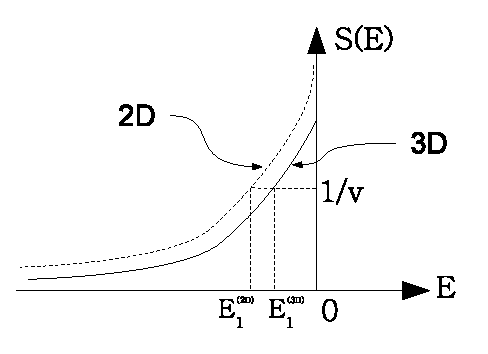
\includegraphics[width=0.30\textwidth]{OnePair.eps}
	\caption{$S^\td(E)$ and $S^{\sd}(E)$ function}
	\label{fig:OnePair}
\end{figure}
whatever $v$. Indeed $S^{(\text{2D})}(E)$ diverges when $E\rightarrow{}0_{-}$ while it goes to zero as $\rho\Omega/(-E)$ when $E$ goes to $-\infty$ as $\rho\Omega/(-E)$. A bound state $E_1<0$solution of Eq. (\ref{eq:s1pair}), thus exists no matter how weak $v$ is. It is given by 
\begin{equation}
E_1^{(\text{2D})}=-\frac{2\sigma}{1-\sigma}\Omega
\label{eq:}
\end{equation}
where we have set $\sigma=e^{-2/\rho{v}}$



\subsection{One pair in 3D systems}
In 3D, the density of states increases as $\sqrt{\epsilon}$. It is convenient to scale it as 
\begin{equation}
\rho(\epsilon)=\rho\sqrt{\epsilon/\Omega}
\label{eq:}
\end{equation}
where $\rho$ is the density of state at the potential threshold. As for 2D systems, this quantity is proportional to the sample volume.   Using this density of state we find
\begin{equation}
\begin{split}
S^\sd(E<0)&=\rho\int_0^{\Omega}{}d\epsilon\frac{\sqrt{\epsilon/\Omega}}{2\epsilon-E}\\
	&=\rho(1-\sqrt{\frac{-E}{2\Omega}}\Arctg\sqrt{\frac{2\Omega}{-E}})
\label{eq:}
\end{split}
\end{equation}


$S^\sd(E)$ goes to $\rho$ when $E\rightarrow0_-$ while it goes to zero as $\frac{2}{3}\rho\Omega/(-E)$ when $E$ goes to $-\infty$. 

A bound state with $E_1<0$ thus exists for $v$ larger than a threshold value for a single pair, $N=1$, given by  $v_{\text{th}}(N=1)=1/\rho$.  For a potential just above threshold, the single pair energy in 3D tends to zero as 
\begin{equation}
E_1^\sd\approx-\frac{8}{\pi^2}\left(1-\frac{1}{\rho{}v}\right)^2\Omega
\label{eq:}
\end{equation}
while for a potential far above threshold $E_1^\sd$ behaves as 
\begin{equation}
E_1^\sd\approx-\frac{2}{3}\rho{v}\Omega
\label{eq:}
\end{equation}


\section{N pairs\label{sec:NPair}}
Richardson \cite{Richardson1} and Gaudin \cite{gaudin} have shown that the energy of $N$ fermion pairs interacting through the BCS reduced potential \emph{with $N_0$  pairs in the frozen Fermi sea core} is exactly given by $E_N=R_1+\cdots+R_N$ where the $R_i$'s follow from $N$ coupled nonlinear equations 
\begin{multline}
 1=v\sum_\vk\frac{w_\vk}{2\epsilon_\vk-R_i}+\sum_{j\neq{}i}\frac{2v}{R_i-R_j}\\\text{for}\;i=(1,\cdots,N)
\end{multline}
\subsection{$N$ pairs in 2D systems}
Very recently, we have shown that when the density of states is constant, as in standard BCS superconductivity but also in 2D systems, a compact form of $E_N$ exists, which reads as  
\begin{equation}
 E^\td_N=N\,E^\td_1+\frac{N(N-1)}{\rho}\frac{1+\sigma}{1-\sigma}
\end{equation}
within under-extensive terms in $(N/\rho)^n$ with $n\leq2$. So that these terms do not appear in thermodynamical limit, as in the ??? canonical approach to the BCS condensation energy. 

This gives the condensation energy per  pairs, i.e., the difference between the $N$-pair energy without and with potential, decreased by the number of pairs, as 
\begin{equation}
 \mathcal{E}^{(2D)}_N=E_N^{\td}(v=0)-E_N^\td\equiv{}N\epsilon_N^\td
 \end{equation}
 So that the condensation energy per pair reduces in 2D to
 \begin{equation}
\epsilon^{(2D)}_N=(1-\frac{N-1}{N_\Omega})\frac{2\sigma}{1-\sigma}\Omega\label{eq:E2D}
\end{equation}
where $N_\Omega=\rho\Omega$ is the total number of states in the potential layer. 

We see that in 2D system, the condensation energy per pair $\epsilon^\td_N$  decreases linearly with $N$ over the whole density range. This decrease is due to a moth-eaten effect induced by Pauli blocking on the number empty states feeling the potential and thus available to from the $N$-pair bound state.  When the number of pairs is large enough to fill the potential layer, $N=N_\Omega$, the condensation energy per pair reduces to 
\begin{equation}
 \epsilon^\td_{N_\Omega}=[\frac{2\sigma}{1-\sigma}]/\rho
\end{equation}
so that it tends to zero as $1/\rho$ in the large sample limit: for $N=N_\Omega$, the system has no more freedom to construct a lower energy ground state, this is why the condensation energy per pair has to cancel.  


\begin{figure}[htbp]
	\centering
		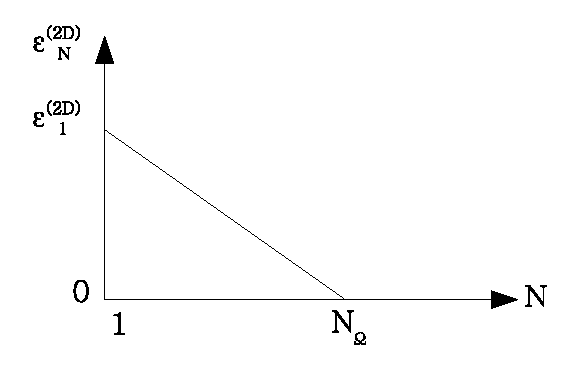
\includegraphics[width=0.30\textwidth]{2dCondEnergy.eps}
	\caption{Condensation energy per pair as a function of the pair number in 2D system}
	$N_{\Omega}$ is the total number of pair state in the potential layer
	\label{fig:2dCondEnergy}
\end{figure}



\subsection{$N$ pairs in 3D system}
Unfortunately, a similar compact expression of the $N$-pair energy has not been derived so far in the case of a $\sqrt{\epsilon}$ density of states. We are thus mostly led with a qualitatively understand of the $N$ pair energy  behavior when $N$ increases. 

First, it is clear that the same moth-eaten effect must bring the condensation energy per pair down to zero when $N$ approach $N_\Omega$: this effect is fundamentally linked to  Pauli blocking , so that it must stand unaffected by an increase of space dimensionality. 

\subsubsection{Qualitative understanding}
For a potential $v$ lower than the threshold value for single pair $v_{th}(1)=1/\rho$, we know that $\mathcal{E}_N^\sd$ is equal to zero for $N=1$ and also for $N=N_\Omega$.  It is however clear that $\mathcal{E}_N^\sd$ cannot stay equal to zero for all $N$ between $1$ and $N_\Omega$ because when $N$ becomes equal to a fraction of $N_\Omega$, the density of states is essentially constant.  So that we can at least freeze a fraction of the $N$ electrons as in standard BCS superconductivity with a frozen core: a finite condensation energy has then appears no matter how weak $v$ is. 

\begin{figure}[htb]
	\centering
		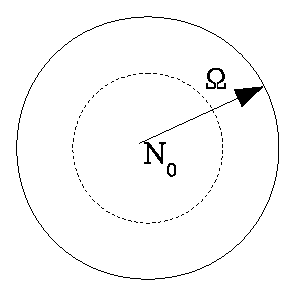
\includegraphics[width=0.20\textwidth]{potential.eps}
	\caption{Effective frozen core in the case of many pairs in 3D system}
	\label{fig:potential}
\end{figure}

To have an estimate of this condensation energy, let us freeze $N_0$ of these $N$ electrons, $\epsilon_{F_{0}}$ being the corresponding Fermi energy.  The remaining $N-N_0$ pairs enjoy the potential attraction in a region where the density of state stays finite, between $\rho\sqrt{\epsilon_{F_0}/\Omega}$ and $\rho$.  The condensation energy of these $(N-N_0)$ pairs would then read according to Eq. (\ref{eq:E2D})
\begin{equation}\label{eq:E3D}
{\mathcal{E}}_{N-N_0}=(N-N_0)(1-\frac{N-N_0-1}{N_\Omega})\frac{2\bar\sigma}{1-\bar\sigma}\Omega
\end{equation}
where $\bar{\sigma}=e^{-2/{\bar{\rho}v}}$ with $\bar\rho$ being the average density of states in the potential layer above the frozen core that we are going to approximate by $\rho$. This gives a  condensation energy for $N-N_0=N_\Omega/2$, which of course implies  $N$ substantially larger than $N_\Omega/2$.

This argument essentially shows that, even if $N$ is not as large as $N_\Omega/2$, but still a sizable faction of the total number of pair state $N_\Omega$ feeling the potential,  a BCS-like collective effect  must take place to produce a non-zero condensation energy, no matter how weak the potential is, i.e., even for $v\ll{}v_\text{th}(1)$. 

As a result, the threshold potential for the appearance of a condensation energy in $N$ pairs  must decrease with $N$, down to essentially zero with $N$ is a sizable fraction of the total number of pairs $N_\Omega$ in the potential layer. 

\begin{figure}[htb]
	\centering
		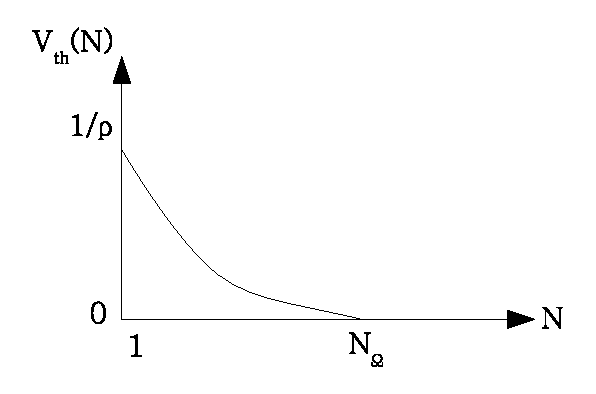
\includegraphics[width=0.30\textwidth]{3dThresholdChange.eps}
	\caption{Threshold change against number of pairs in 3D}
	\label{fig:3dThresholdChange}
\end{figure}

\subsubsection{}
For $v$ above the threshold value $v_{\text{th}}(1)=1/\rho$ for the appearance of bound state in the case of only one pair, it becomes  clear by continuity, that the condensation energy per pair $\epsilon^\sd_N$, must first increases with $N$ and then decreases due to the moth-eaten effect which must end by controlling the behavior of $\epsilon_N$ when $N$ approaches full filling.  Although fully reasonable, the above continuity argument is, when $v$ gets above $v_{\text{th}}(1)$ is a mathematical argument, not a physical argument. 

It is actually possible to grasp the physical origin of the condensation energy increase when $N$ departs from 1.  It mainly comes from the free fermion continuum.  For that, we have to remember that the condensation energy is the difference of two energies which both increase with $N$ due to Pauli blocking.  The question then is to understand why, for small $N$, the free pair energy increases faster than the correlated pair energy.  When one free pair is added at the energy level $\epsilon$, the kinetic energy increases by $1/\rho(\epsilon)$.  As a result, in 3D systems with density of states in $\sqrt{\epsilon}$, the free pair energy change when going from $N$ to $N+1$ pairs, is very large when the Pauli exclusion principle blocks a low energy state.  By contrast, correlated pairs are made of all pairs in the potential layer. When increasing their number from $N$ to $N+1$, we blocks a very small fraction of each of the states between $0$ and $\Omega$, so that the energy change must be far less than when blocking a single low energy state.  Consequently the energy difference when adding one free pair on one correlated must increase with $N$ is small. By contrast when $N$ gets larger, the cost in energy $1/\rho(\epsilon)$ to add one free pair is eventually constant and equal to the cost to block any of the $\vk$ states making the correlated pair.  We are then left with the moth-eaten effect on the bound state itself which tends to decrease the condensation energy. 

This understanding is supported by the monotonous decrease of the condensation energy per pair we find in 2D: the density of state being constant, the energy cost to block a single low energy state is the same as for any of the states making the correlated pair so that we only feel the moth-eaten effect on the number of states available to construct the correlated configuration.  As a result, the condensation energy per pair has to decrease without when $N$ increases as we find.  

In order to establish this qualitative understanding on strong grounds, let us consider $N=2$ pairs. This limiting case gives the trend of the $N$ dependence of the condensation energy since it actually contains the physics which drives this $N$ dependence, namely Pauli blocking.  

\begin{figure}[htb]
	\centering
		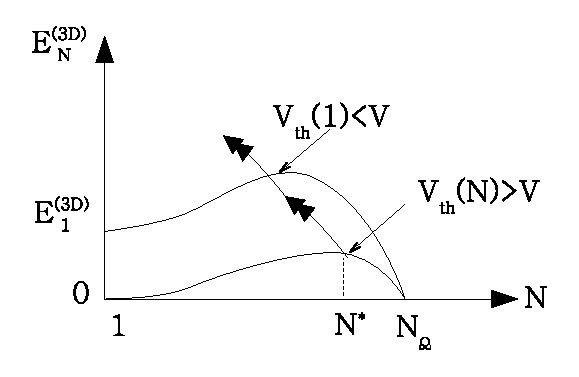
\includegraphics{3dCondChange.eps}
	\caption{Condensation energy change with number of pairs in 3D}
	\label{fig:3dCondChange}
\end{figure}

\section{Condensation energy in two pairs\label{sec:twoPair}}
The exact energy of two fermion pairs in the reduced BCS potential given in Eq. (\ref{eq:VBcs}), has been shown to read as$E_2=R_1+R_2$ where $(R_1,R_2)$ are solution of the two Richardson-Gaudin equations
\begin{equation}
\begin{split}
1&=v\sum_{\vk}\frac{w_\vk}{2\epsilon_\vk-R_1}+\frac{2v}{R_1-R_2}\\
1&=v\sum_{\vk}\frac{w_\vk}{2\epsilon_\vk-R_2}+\frac{2v}{R_2-R_1}
\end{split}
\label{eq:richardsonEq}
\end{equation}

If we now add and subtract these two equations, and use the single pair energy $\epsilon_{1}$ given in  Eq. (\ref{eq:onePair}), we rewrite this set equations without $v$, now hidden in $E_{1}$.  It reads 
\begin{gather}
\begin{split}
0=&(R_1-E_1)\sum_{\vk}\frac{w_\vk}{(2\epsilon_\vk-R_1)(2\epsilon_\vk-E_1)}\\
&+(R_2-E_1)\sum_{\vk}\frac{w_\vk}{(2\epsilon_\vk-R_2)(2\epsilon_\vk-E_1)}\label{eq:2PairPlus}
\end{split}\\
-\frac{4}{(R_1-R_2)^2}=\sum_{\vk}\frac{w_\vk}{(2\epsilon_\vk-R_1)(2\epsilon_\vk-R_2)}\label{eq:2PairMinus}
\end{gather}

\subsection{Two pairs in 2D systems}
We have been able to solve these coupled equations analytically in the BCS case of a constant density of states and a frozen Fermi sea\cite{combescotBCS}.  We can use  this work,  for 2D systems having a constant density of state but write now $w_\vk=1$ for $0<\epsilon_k<\Omega$. The energy difference between two correlated pairs and two independent pairs reads in the large sample limit, as 
\begin{equation}
E^{\td}_2-2E_1^{\td}=\frac{2}{\rho}\left(1+\frac{2\sigma}{1-\sigma}\right)+\text{O}(\frac{1}{\rho^2})
\label{eq:}
\end{equation}
the $2/\rho$ contribution is the kinetic energy cost to add one pair when the density of state is constant while $2[2\sigma/(1-\rho)]$ is the change in the binding energy of two pairs induced by the moth-eaten effect. This result far easier to obtain than the one for arbitrary $N$, not only gives the trend induced by Pauli blocking on the energy of $N$ correlated pairs, but also allows to obtain this energy exactly through a rule of the thumb that we have learned valid for all exciton problems we have studied up to now - excitons also being composite bosons with a many-body physics fully driven by Pauli blocking.  This rule says that, in the thermodynamical limit, i.e., large volume but $N/\rho$ constant, the result for $N$ is the result in 2 multiplied by $N-1$.  In the present case, this gives the energy change per pair, $[E^{\td}_N-NE^{\td}_1]/N$, as $[(N-1)/\rho](1+\sigma)/(1-\sigma)$ in agreement with the result we have found through a far more complicated procedure than the ones to obtain the result in $N=2$.

\subsection{Two pairs in 3D system}
We now look in solution of these two equations when the density of states is not constant but varies as $\rho\sqrt{\epsilon/\Omega}$.  Since the solution of these equations for $N=1$, i.e., without the $2v/(R_1-R_2)$ terms in Eq. (\ref{eq:richardsonEq}), dramatically depends on the values of $\rho{}v$ compared to 1, with no bound state, i.e., negative solution, if $v$ is smaller than $v_{\text{th}}(1)=1/\rho$. We are led to consider the three cases $v\rho>1$, $v\rho<1$ and $v\rho=1$ separately. 

We notice that a property of the $R_i$'s we have found in our previous work (see sec. IIIB of ref. \cite{combescotBCS}), is still valid whatever $\rho{}v$ is, namely the fact that $R_1$ and $R_2$ are both complex with $R_1=R_2^*$.% in order to have $R_1+R_2=E_2$ real.  
%Let us first reproduce the argument in completeness. 

%\subsection{$(R_1,R_2)$ are complex conjugate}
%Let us write $R_{1,2}=R\pm{}iR'$, and we need to show that $R$ and $R'$ are real.  First, we notice that $R$ must be real as $2R=E_{2}=R_{1}+R_{2}$ is the energy of the Hamiltonian, which is hermition operator, and must be real. 

\subsubsection{Solution in $v\rho>1$}
Let us first consider  $v\rho>1$.  A single pair then have a well defined bound state with $E_1$ is finite. Since the change between the two pair energy $R_{1}+R_{2}$ and two single pair energy $2E_{1}$ can only come from Pauli blocking due to the very peculiar form of the reduced BCS potential, we expect $R_1+R_2\approx2E_1$, when $L^3\rightarrow\infty$, i.e., when $\rho\rightarrow\infty$. Eq. (\ref{eq:2PairPlus}) then leads to  
\begin{equation*}
0\approx(R_1+R_2-2E_1)\sum\frac{w_\vk}{(2\epsilon_\vk-E_1)^2}
\label{eq:}
\end{equation*}
which confirms  $R_1+R_2\approx2E_1$, i.e.,  $R_1\approx{}R_2\approx{}E_1$ at lowest order in $1/\rho$ since the sum over $\vk$ increase with sample volume as   
\begin{equation}
\begin{split}
I_n&=\sum_{\vk}\frac{w_\vk}{(2\epsilon_\vk-E_1)^{n+1}}\\
	&=\frac{\rho}{\Omega}\int^1_0\frac{\sqrt{x}dx}{(2x-E_1/\Omega)^{(n+1)}}\\
	&\equiv\frac{\rho}{\Omega}g_n(E_1/\Omega)
\end{split}
\label{eq:}
\end{equation}
To go further, we use Eq. (\ref{eq:2PairMinus}). It gives 
\begin{equation}
-\frac{4}{(R_1-R_2)^2}\approx\sum_{\vk}\frac{w_\vk}{(2\epsilon_\vk-E_1)^2}=I_1
\label{eq:}
\end{equation}


%And this gives 
%\begin{equation}
%R_1-R_2\approx{}i\frac{\Omega}{\sqrt{\rho\Omega{}g_1(E_1/\Omega)}}
%\label{eq:}
%\end{equation}

If we now keep to terms in to Eq. (\ref{eq:2PairPlus}), namely
\begin{equation}
\begin{split}
0=&(R_1-E_1)\sum{\frac{w_\vk}{(2\epsilon_\vk-E_1)}}\\
&\left(\frac{1}{2\epsilon_\vk-E_1}+\frac{1}{2\epsilon_\vk-R_1}-\frac{1}{2\epsilon_\vk-E_1}\right)\\
&+(R_1\leftrightarrow{}R_2)
\end{split}
\end{equation}
We can rewrite this equation as
\begin{equation}
\begin{split}
0\approx&(R_1-E_1+R_2-E_1)I_1\\
&+\left[(R_1-E_1)^2+(R_2-E_1)^2\right]I_2\\
=&(R_1-E_1+R_2-E_1)I_1\\
&+\left[(R_1+R_2-E_1)^2+(R_2-R_1)^2\right]\frac{I_2}{2}
\end{split}
\label{eq:}
\end{equation}
which reduces  to 
\begin{equation}
R_1-E_1+R_2-E_1\approx-\frac{I_2}{2I_1}(R_2-R_1)^2=\frac{2I_2}{I_1^2}
\label{eq:}
\end{equation}
So the two pair energy reads as
\begin{equation}
R_1+R_2=2E_1+2\frac{\Omega}{\rho}\frac{g_2(E_1/\Omega)}{g_1^2(E_1/\Omega)}
\label{eq:}
\end{equation}
If we assume $g_n(E_1/\Omega)$ is in order of 1, we see the increase of binding energy (moth-eaten effect) is in order of $O(\frac{1}{\rho})$.  On the other hand, increase in energy of free Fermi gas is in the order of density of state, which is in order of $\rho^{-\frac{2}{3}}$, which is far larger than increase before.  Therefore, the condensation energy increases. This can be understand more intuitively as such: a tight-binding state occupies large momentum-space with very small weight on each level. Therefore, Pauli blocking when introducing an extra pair is quite small as the occupation is much smaller than 1. Therefore, it is better energetically to put two pairs both in a state very like the original single-pair bound state than simply put the second pair in the next highest k-level as free Fermi gas.   
\subsubsection{Solution in $v\rho=1$}
Let us start with the threshold case $v=v_{\text{th}}(1)$, i.e., $v\rho=1$.  We then have $S(E=0)=1$, so that the Richardson-Gaudin equations also read, for $R_1=R+iR'$
\begin{equation}
\sum\frac{w_\vk}{2\epsilon_\vk}=\sum\frac{w_\vk}{2\epsilon_\vk-R-iR'}-\frac{i}{R'}
\label{eq:}
\end{equation}
This equation splits into two equations, for the real and imaginary parts

The problem then is to find $R$ solution of 
\begin{equation}
\sum\frac{w_\vk}{2\epsilon_\vk}=\sum{}w_\vk\frac{2\epsilon_\vk-R}{(2\epsilon_\vk-R)^2+R'^2}
\label{eq:}
\end{equation}
where $R'$ such that 
\begin{equation}
R'^2\sum{}\frac{w_\vk}{(2\epsilon_\vk-R)^2+R'^2}=1
\label{eq:R'}
\end{equation}
in the large sample limit, i.e., the dominate term of the $\rho$ dependence of $R$ when $1/\rho$ goes to zero. 

By combining these two equation, we get
\begin{equation}
R\sum{}w_\vk\frac{2\epsilon_\vk-R}{(2\epsilon_\vk-R)^2+R'^2}=1
\label{eq:R}
\end{equation}

A possible trick to solve these equations is to note that $\sum_\vk{}w_\vk=N_\Omega=\frac23\rho\Omega$ in 3D (which it is $\rho\Omega$ in 2D).  This allows to rewrite Eqs. (\ref{eq:R'},\ref{eq:R})
\begin{gather}
\sum{}w_\vk\left[\frac{1}{(2\epsilon_\vk-R)^2+R'^2}-\frac{1}{N_\Omega{}R'^2}\right]=0\\
\sum{}w_\vk\left[\frac{2\epsilon_\vk-R}{(2\epsilon_\vk-R)^2+R'^2}-\frac{1}{N_\Omega{}R}\right]=0
\end{gather}
This readily shows that if $R$ and $R'$ were finite when $\rho\rightarrow\infty$, i.e., these questions cannot be fulfilled because we 
................................



\section{Conclusion\label{sec:conclusion}}
The upper energy cutoff $\Omega$ for the phase space in our model seems quite arbitrary.  After all, real system has no such cutoff and they have infinite amount of high-momentum states to use.   It seems a little dubious that condensation energy vanishes when all states below $\Omega$ is filled.  On the other hand, this fact can be interpret in such way:  energy cutoff $\Omega$ is introduced because we take potential as constant and ignore the fall-off of the potential in high energy.  The amplitude of potential defines an energy scale, which in turn defines a region in phase space.  Beyond this space, potential is too small and does not affect the distribution of fermions and fermions pack themselves just as free gas, therefore equivalently gives zero condensation-energy. 

We present an analysis about the transition from one-pair and many-pair with the same hamiltonian within Richardson-Gaudin equations framework.  We observe that condensation energy increases in the beginning and decreases toward the full filling. When attraction is small enough, there is no bound state for single pair, but later, fermions formed a many-body bound state and lower the system energy, when fermion number further increases, system gets back into the normal state as free Fermi gas.  By utilizing Richardson-Gaudin equations in canonical ensemble, we illustrate the intricacy of the many-body state of superconductivity.  

One of us (M.C.) wishes to thank the University of Illinois at
Urbana-Champaign, and Tony Leggett in particular, for enlightening discussions during her invitations at
the Institute for Condensed Matter Physics where most of the present work has been
performed. 

%\bibliographystyle{apsrmp4-1long}
\bibliographystyle{unsrt}
\bibliography{../citation}

\end{document}
